%
% Modelo de relatório/trabalho
%
\documentclass[a4paper, 12pt]{article}

\usepackage[english]{babel}
\usepackage[utf8]{inputenc}
\usepackage[T1]{fontenc}
\usepackage{fontspec}
\usepackage{array}
\usepackage{fixltx2e}
\usepackage{amsmath}
\usepackage{amssymb}
\usepackage{graphicx}
\usepackage{subcaption}
\usepackage{float}
\usepackage{a4wide}
\usepackage{array}
\usepackage{multicol}
\usepackage[table]{xcolor}
\usepackage{makeidx}
\usepackage{hyperref}
\usepackage{booktabs}
\usepackage{setspace}
\usepackage{minted}
\usepackage[bottom]{footmisc}
\usepackage[nottoc]{tocbibind}
\usepackage{listings}
\usepackage[a4paper]{geometry}
\usepackage[square, sort, comma, numbers]{natbib}

\onehalfspacing
\graphicspath{{./img/}}

\setcounter{secnumdepth}{2}
\setcounter{tocdepth}{2}

\setsansfont{DejaVu Sans}
\setmonofont{DejaVu Sans Mono}

\begin{document}

\hypersetup{backref,pdfpagemode=FullScreen,colorlinks=true}

\thispagestyle{empty}
\begin{center}
    \textbf{\Large{Autotuning with Cloud Computing}}\\

    \vspace*{0.5cm}

    \begin{minipage}{.3\linewidth}
        \begin{flushleft}
            Pedro Bruel\\
            phrb@ime.usp.br
        \end{flushleft}
    \end{minipage}
    \begin{minipage}{.3\linewidth}
        \begin{center}
            Alfredo Goldman\\
            gold@ime.usp.br
        \end{center}
    \end{minipage}
    \begin{minipage}{.3\linewidth}
        \begin{flushright}
            Daniel Batista\\
            batista@ime.usp.br
        \end{flushright}
    \end{minipage}

    \vskip 0.5cm

    \normalsize{Instituto de Matemática e Estatística (IME)\\
                Universidade de São Paulo (USP)\\
                R. do Matão, 1010 – Vila Universitária, São Paulo – SP, 05508-090\\}

\end{center}

\begin{abstract}
This research project presents a proposal for a conference paper.
The objective is to extend the OpenTuner autotuning framework to
leverage the cloud computing resources from Google Compute Engine.
An overview of the autotuning research area is presented,
supporting the novelty and contribution potential of this proposal.
The objectives and current work are discussed in detail, and a research
schedule is presented.
\end{abstract}

\section{Introduction} \label{sec:intro}

The program autotuning problem fits in the framework of the Algorithm Selection
Problem, introduced by Rice in 1976~\cite{rice1976algorithm}. The objective of
an autotuner is to select the best algorithm, or algorithm configuration, for
each instance of a problem.  Algorithms or configurations are selected
according to performance metrics such as the time to solve the problem
instance, the accuracy of the solution and the energy consumed.  The set of all
possible algorithms and configurations that solve a problem define a
\emph{search space}. Guided by the performance metrics, various optimization
techniques search this space for the algorithm or configuration that best
solves the problem.

\begin{figure}[htpb]
    \centering
    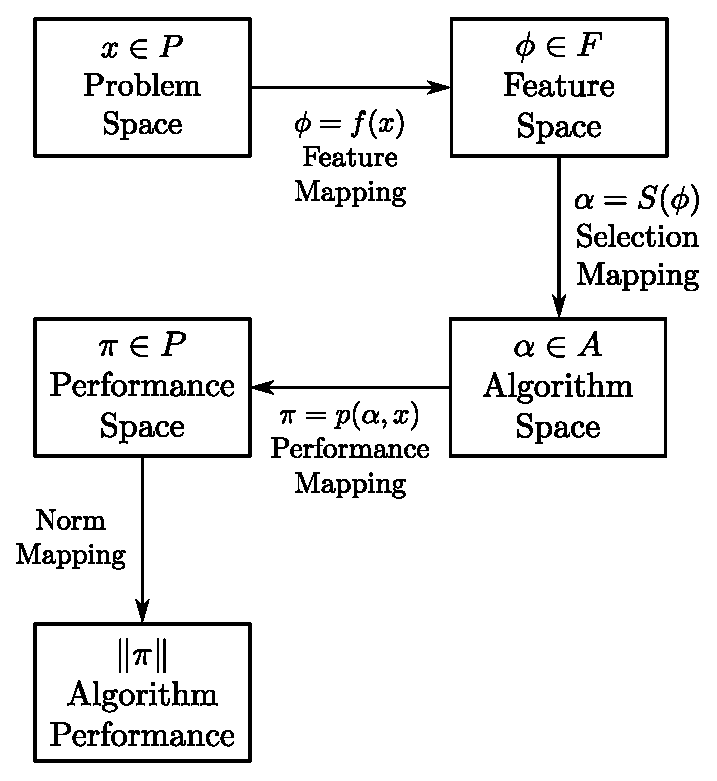
\includegraphics[scale=.5]{algorithm-selection}
    \caption{Rice's Algorithm Selection Framework~\cite{rice1976algorithm}.}
    \label{fig:asf}
\end{figure}

Autotuners can specialize in domains such as matrix
multiplication~\cite{bilmes1997phipac}, dense~\cite{whaley1998atlas} or
sparse~\cite{vuduc2005oski} matrix linear algebra, and parallel
programming~\cite{jordan2012multi}. Other autotuning frameworks provide more
general tools for the representation and search of program configurations,
enabling the implementation of autotuners for different problem
domains~\cite{ansel2014opentuner,hutter2009paramils}.

Figure~\ref{fig:asf} shows the Algorithm Selection Problem framework.
Bougeret \emph{et al.}~\cite{bougeret2009combining} proved that the Algorithm
Selection Problem is NP-complete when calculating static distributions of
algorithms in parallel machines.  Guo~\cite{guo2003algorithm} proved the
problem is undecidable in the general case.

This research proposal consists in the implementation of an
extension to the OpenTuner framework~\cite{ansel2014opentuner} that will
enable it to leverage cloud computing resources.
The remaining of this document is organized as follows.
Section~\ref{sec:related} discusses related work and the OpenTuner
framework.
Section~\ref{sec:obj} presents a detailed discussion of the objectives
and reports the current state of the research.
Section~\ref{sec:exp} discusses the methods and benchmarks that will be used to
test and validate the implementations.
Section~\ref{sec:sched} presents a preliminary schedule.
Section~\ref{sec:conclusion} concludes the proposal.

\section{Related Work} \label{sec:related}

Rice's conceptual framework~\cite{rice1976algorithm} formed the foundation
of autotuners in various problem domains.  In 1997, the PHiPAC
system~\cite{bilmes1997phipac} used code generators and search scripts to
automatically generate high performance code
for matrix multiplication. Since then, systems tackled different domains with a
diversity of strategies. Whaley \emph{et al.}~\cite{whaley1998atlas} introduced
the ATLAS project, that optimizes dense matrix multiply routines. The
OSKI~\cite{vuduc2005oski} library provides automatically tuned kernels for
sparse matrices. The FFTW~\cite{frigo1998fftw} library provides tuned C
subroutines for computing the Discrete Fourier Transform.  In an effort to
provide a common representation of multiple parallel programming models, the
INSIEME compiler project~\cite{jordan2012multi} implements abstractions for
OpenMP, MPI and OpenCL, and generates optimized parallel code for heterogeneous
multi-core architectures.

Some autotuning systems provide generic tools that enable the implementation of
autotuners in various domains. PetaBricks~\cite{ansel2009petabricks} is a
language, compiler and autotuner that introduces abstractions, such as the
\texttt{\footnotesize either...or} construct, that enable programmers to define
multiple algorithms for the same problem.  The ParamILS
framework~\cite{hutter2009paramils} applies stochastic local search methods
for algorithm configuration and parameter tuning.  The OpenTuner
framework~\cite{ansel2014opentuner} provides ensembles of techniques that
search spaces of program configurations. Bosboom \emph{et al.} and Eliahu use
OpenTuner to implement a domain specific language for data-flow
programming~\cite{bosboom2014streamjit} and a framework for recursive parallel
algorithm optimization~\cite{eliahu2015frpa}.

In a progression of papers~\cite{gupta2012exploring,gupta2014evaluating,gupta2013hpccloud},
Gupta \emph{et. al} provide experimental evaluations of the application of
cloud computing to high performance computing, describing which kind of
applications has the greatest potential to benefit from cloud computing.
Their work highlights small and medium scale projects as the main beneficiaries
of cloud computing resources.

\subsection{OpenTuner} \label{sec:opt}

OpenTuner search spaces are defined by \emph{Configurations}, that are composed
of \emph{Parameter} of various types. Each type has restricted bounds and
manipulation functions that enable the exploration of the search space.
OpenTuner implements ensembles of optimization techniques that
perform well in different problem domains. The framework uses
\emph{meta-techniques} to coordinate the distribution of resources
between techniques.
Results found during search are shared between techniques through a
database. An OpenTuner application can implement its own search
techniques and meta-techniques, making the ensemble more robust.

\begin{figure}[htpb]
    \centering
    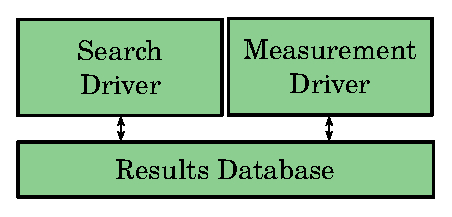
\includegraphics[scale=.62]{opentuner-implementation}
    \caption{Simplified OpenTuner Architecture.}
    \label{fig:ot-imp}
\end{figure}

Figure~\ref{fig:ot-imp} shows a high-level view OpenTuner's architecture.
Measurement and searching are done in separate modules, called drivers,
that share results through the database. The search driver requests
measurements by registering configurations to the database. The measurement
driver reads those configurations and writes back the desired results.
Currently, the measurements are performed sequentially.

OpenTuner implements optimization techniques such as the
Nelder-Mead~\cite{nelder1965simplex} simplex
method and Simulated Annealing~\cite{kirkpatrick1983optimization}.
OpenTuner implements a resource sharing mechanism that aims to take
advantage of the strengths of each technique. A meta-technique
must balance the exploitation of a technique that has produced
good results in the past and the exploration of new, and possibly
best, techniques.

\section{Objectives} \label{sec:obj}

The objectives of this research project are the following:

\begin{itemize}
    \item Implement an extension to the OpenTuner measurement driver,
        the \emph{MeasurementClient}, that requests virtual
        machines in the Google Compute Engine to produce
        measurements of configurations;
    \item Implement a \emph{MeasurementServer} that runs
        in the virtual machines. The server receives
        requests for results, computes them, and send
        them to the client;
    \item Normalize the results obtained from virtual machines
        to the local machine;
    \item Evaluate the performance of the implementation,
        using the benchmark applications provided with
        OpenTuner~\cite{ansel2014opentuner}.
\end{itemize}

The remaining of this section describes the implementation objectives in
detail, and reports the current state of the research. Section~\ref{sec:exp}
describes the performance evaluations and the benchmark.

\subsection{Measurement Server and Client}

The interactions between the local and virtual machines
will follow the client-server model. The local machine
will run a measurement client, that will request
results from various measurement servers running in
virtual machines hosted at the Google Compute Engine.

Figure~\ref{fig:high-level} shows the proposed architecture
of an OpenTuner application running the measurement
client and communicating with the measurement servers.
Green boxes in the figure represent OpenTuner modules
that will not be modified, and blue boxes represent
new or modified modules.

Figure~\ref{fig:low-level} shows, on a lower level
of abstraction, the interactions between the measurement
client and servers. A simple application protocol
will be devised to mediate the requests and responses.
The configurations will be sent to the server, that
will run the correspondent program and respond with
the measurement.

\begin{figure}[htpb]
    \centering
    \begin{subfigure}{.45\textwidth}
        \centering
        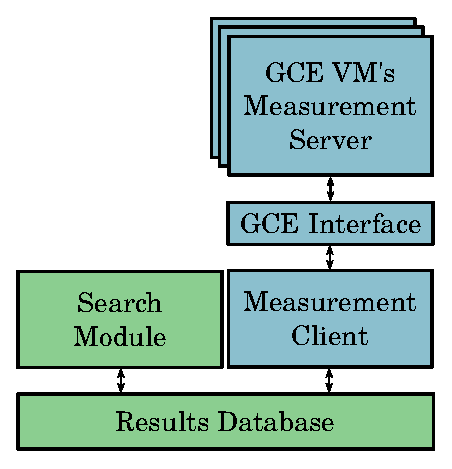
\includegraphics[scale=.62]{high-level-implementation}
        \caption{A high-level view of the proposed architecture.
        Green boxes represent unmodified modules, blue boxes represent
        new or modified modules.}
        \label{fig:high-level}
    \end{subfigure}%
    \hfill
    \begin{subfigure}{.45\textwidth}
        \centering
        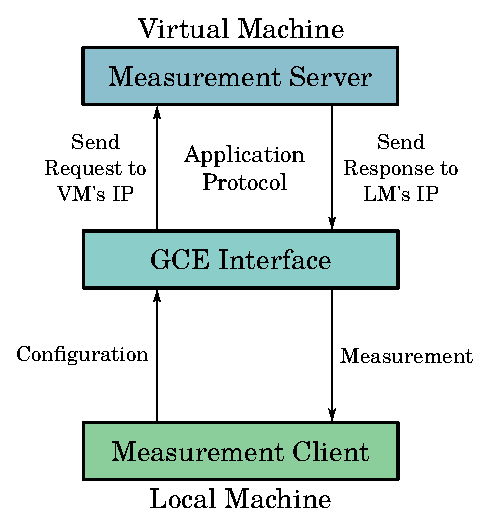
\includegraphics[scale=.62]{low-level-implementation}
        \caption{A lower-level view of the proposed architecture,
        Illustrating the communication between server and client,
        mediated by the Google Compute Engine API.
        }
        \label{fig:low-level}
    \end{subfigure}%
    \caption{Proposed OpenTuner Architecture,
    using the Google Compute Engine (GCE) API.}
    \label{fig:archs}
\end{figure}

OpenTuner controls the execution flow of an application
with the \texttt{\footnotesize main} function of the
\texttt{\footnotesize TuningRunMain} class. This function
calls the \texttt{\footnotesize main} function of the
search driver, which runs the main loop of an OpenTuner
application. The search driver generates configurations
to be tested and saves them to the database. It them calls
the \texttt{\footnotesize process\_all} function of the
measurement driver and blocks until the function returns.

The measurement driver is able to compile programs in parallel,
but the measurements are done sequentially.
Listing~\ref{fig:measurement-client} shows the functions of
the measurement driver that will have to be modified for the
\texttt{\footnotesize MeasurementClient} to be able to
process results with the Google Compute Engine.

During its initialization, the measurement client will
initialize and configure the virtual machines, storing
each measurement server's IP in the GCE interface.
When the search driver requests for results,
the \texttt{\footnotesize process\_all} function will route
the requests to the servers via the GCE interface.
The interface will call the appropriate GCE Python API
functions to send requests to the servers, and will wait
for their responses.

The OpenTuner source code is
available\footnote{The code is hosted at GitHub:
\texttt{\scriptsize github.com/jansel/opentuner}} under
the MIT License.

\begin{listing}[htpb]
    \begin{minted}[fontsize=\scriptsize]{python}
class MeasurementClient(MeasurementDriver):
    """
    Reads DesiredResults and requests VMs
    in the cloud to compute Results.
    """
    def __init__(self,
           measurement_interface,
           input_manager,
           **kwargs):
        super(MeasurementDriver, self).__init__(**kwargs)
        """
        Now, the client will instantiate and 
        configure the VM Measurement Servers.
        """

    def process_all(self):
        """
        Process all results in the
        database, by sending requests to
        VMs in the cloud and waiting
        responses.
        """
    \end{minted}
    \caption{A simple echo server in Python.}
    \label{fig:measurement-client}
\end{listing}


\subsection{Normalizing the Results}

The autotuner will optimize programs for a machine that will
typically have an architectural specification different
from the machines in the cloud. A normalization technique
must be devised that enables the results found in the
virtual machines to be valid for the local machine.
Four preliminary approaches to this problem are discussed
in the following.

\subsubsection{Use OpenTuner to Model Performance}

Another autotuner could be used to optimize parameters
of a simple performance model, that would associate
a configuration's measurement and the virtual machine
that produced it with a conversion function. This function
should map the performance result to the target architecture,
producing a valid result.

\subsubsection{Compose Ensembles of Virtual Machines}

The cloud application could be composed of virtual machines
with different architectures. The final performance measurement
for a configuration would then be built from the results obtained
in these different virtual machines.

\subsubsection{Simulate the Target Architecture}

The target machine could be modeled by an architecture
simulator such as \emph{zsim}~\cite{sanchez2013zsim},
a simulator for multi-core architectures
available\footnote{Hosted at GitHub: \texttt{\scriptsize https://github.com/s5z/zsim}}
under the GNU General Public License.
Using a simulator would solve the normalization problem but introduce
other problems, such as the simulator's accuracy and performance.

\subsubsection{Run the Autotuner in the Cloud}

Finally, the normalization problem could be sidestepped, at least
in initial research, by running the servers and clients in the cloud
using the same kind of virtual machine.

\subsection{Using the Google Compute Engine} \label{sec:pwork}

Simple experiments with GCE have been performed. A project
was started and utility functions were implemented.
The utilities include adding and removing virtual machines,
configuring firewall access rules, configuring virtual machines
with a startup script and obtaining a virtual machine's IP.

Each virtual machine is setup and starts running a simple
Python TCP echo server at the \texttt{\footnotesize 8080}
port. Figure~\ref{fig:server-test-code} shows the code for the
server.

The utility functions and the measurement server's and client's code
are available\footnote{All code is hosted at GitHub: \\
\texttt{\scriptsize github.com/phrb/measurement-server} \\
\texttt{\scriptsize github.com/phrb/autotuning-gce}}
under the GNU General Public License.

\begin{listing}[htpb]
    \begin{minted}[fontsize=\scriptsize]{python}
#!/usr/bin/env python

import socket

TCP_IP = ''
TCP_PORT = 8080
BUFFER_SIZE = 1024

s = socket.socket(socket.AF_INET, socket.SOCK_STREAM)
s.bind((TCP_IP, TCP_PORT))
s.listen(1)

conn, addr = s.accept()

while 1:
    data = conn.recv(BUFFER_SIZE)
    if not data: break
    conn.send(data)
    \end{minted}
    \caption{A simple echo server in Python.}
    \label{fig:server-test-code}
\end{listing}


\section{Experiments} \label{sec:exp}

A benchmark of applications will be composed to compare the performance of
the OpenTuner framework with and without the proposed modifications.
An ideal benchmark would comprise the applications used to validate
OpenTuner~\cite{ansel2014opentuner}.
The normalization techniques devised for the results from virtual machines
will be compared using the same benchmark.

We expect that the experiments provide insight into the situations
when using cloud computing resources for autotuning is beneficial,
and into the application and efficiency of the result normalization
techniques.

\section{Research Schedule} \label{sec:sched}

Table~\ref{tab:sched} presents a first version of the research schedule
following the assignment's delivery dates.
The schedule spreads the tasks so that portions of the work
predicted to be harder are assigned to longer time frames.

\newcolumntype{K}{>{\centering\arraybackslash}m{3cm}}
\newcommand{\specialcell}[2][c]{%
  \begin{tabular}[#1]{@{}K@{}}#2\end{tabular}}

\begin{table}[htpb]
    \centering
    \scriptsize
    \begin{tabular}{@{}KKKK@{}}
        \toprule
        \specialcell{\bf AP2 \& PR \\ \bf 25/09} & \specialcell{\bf AR1 \\ \bf 16/10} & \specialcell{\bf AP3 \& AR2 \\ \bf 13/11} & \specialcell{\bf AR3 \\ \bf 25/11} \\ \midrule
        \specialcell{ \footnotesize Paper proposal. \\[0.15cm]
            \footnotesize 10-minute presentation. \\[0.15cm]
            \footnotesize Preliminary experiments at GCE. \\[0.15cm]
            \footnotesize High and low-level views of the implementation.}
            & \specialcell{ \footnotesize First version of the paper. \\[0.15cm]
            \footnotesize Measurement Client implementation. \\[0.15cm]
            \footnotesize Result normalization techniques. \\[0.15cm]
            \footnotesize GCE Interface implementation.}
            & \specialcell{ \footnotesize Second version of the paper. \\[0.15cm]
            \footnotesize 20-minute presentation. \\[0.15cm]
            \footnotesize Measurement Server implementation. \\[0.15cm]
            \footnotesize Application protocol specification.}
            & \specialcell{ \footnotesize Final version of the paper. \\[0.15cm]
            \footnotesize Experiments, results and analysis.} \\ \bottomrule
    \end{tabular}
    \caption{Task scheduling for the project.}
    \label{tab:sched}
\end{table}

\section{Conclusion} \label{sec:conclusion}

\bibliographystyle{plainnat}
\bibliography{ref}

\end{document}
